\documentclass[border=3pt,tikz]{standalone}
\usetikzlibrary{angles,quotes}
\begin{document}
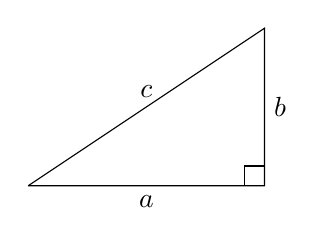
\begin{tikzpicture}[x=1cm,y=1cm]
  \coordinate (A) at (1.5,-1);
  \coordinate (B) at (1.5,1);
  \coordinate (C) at (-1.5,-1);
  \draw (C) -- node[above] {$c$} (B) -- node[right] {$b$} (A) -- node[below] {$a$} (C);
  \draw (A) +(-.25,0) |- +(0,.25);
\end{tikzpicture}
\end{document}